\section{Target group analysis}\label{sec:target-group-analysis}

Chess as a game has a broad appeal, as it is played by many people, young and old.
As previously stated, chess has risen in popularity recently, so it is sufficed to say that the user group is a lot
larger than it was a few years ago.
Therefore, it is necessary to analyze the target group to narrow down the scope of the project.

A good way to do just that is by splitting the target group into different categories.
It is possible to split the people that play chess by age, skill level, and how frequently they play.
As the project is about the learning process of chess, dividing the target group by skill level is the most relevant.
In that case, our target group is novices and beginners.

% textidote: ignore begin
\begin{figure}
    \centering
    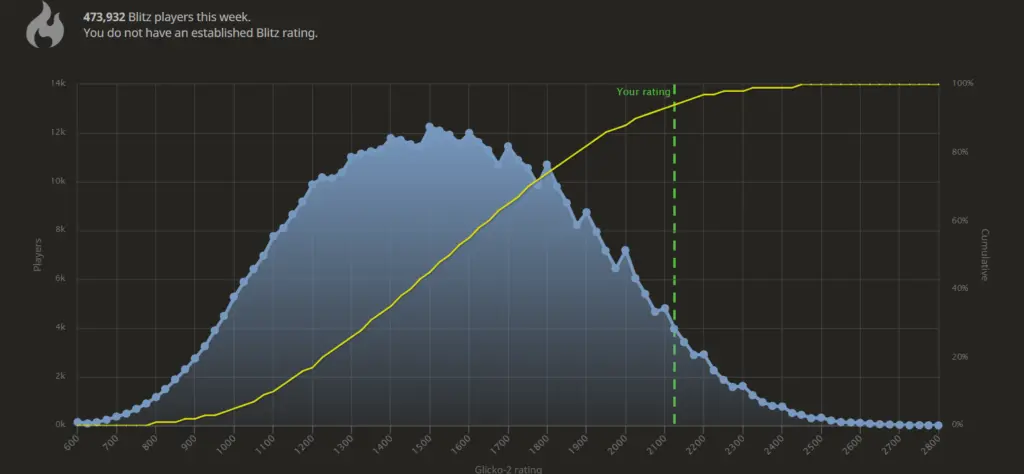
\includegraphics[width=0.75\textwidth]{lichess-rating}
    \caption{Lichess rating system~\cite{chess-ratings}.}\label{fig:lichess-rating}
\end{figure}

\begin{figure}
    \centering
    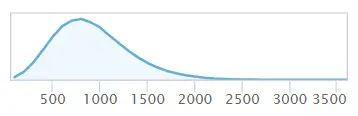
\includegraphics[width=0.5\textwidth]{chess-rating}
    \caption{Chess.com rating system~\cite{chess-ratings}.}\label{fig:chess.com-rating}
\end{figure}

% textidote detects chess.com as an error, whitelisting it doesn't seem to work

The Figure~\ref{fig:lichess-rating} shows a graph of the player base of Lichess.
Unlike in Chess.com's data in Figure~\ref{fig:chess.com-rating}, Lichess has a more detailed graph of the player base,
because it gives a percentage of the player base and their rating.
ChessGoals lists Chess.com scores below 1100 as beginners~\cite{chess-ratings}, but it's visible from the graph that
the rating systems are not directly interchangeable.
% textidote: ignore end
By comparing and aligning the two graphs, it is possible to estimate a rating under 1500 as beginners for Lichess.
Referencing the graph, it can be concluded that 45\% of the chess player base are beginners.

This is a pretty big proportion, given that most of the digital chess platforms are designed for experienced players.
Therefore, it can be concluded that there is a need for a platform that is designed for beginners.
